\documentclass{standalone}
\usepackage{tikz}

\definecolor{viridisblue}{RGB}{68,1,84}
\definecolor{viridisyellow}{RGB}{253,231,37}
\definecolor{viridisgreen}{RGB}{35,138,141}

\begin{document}

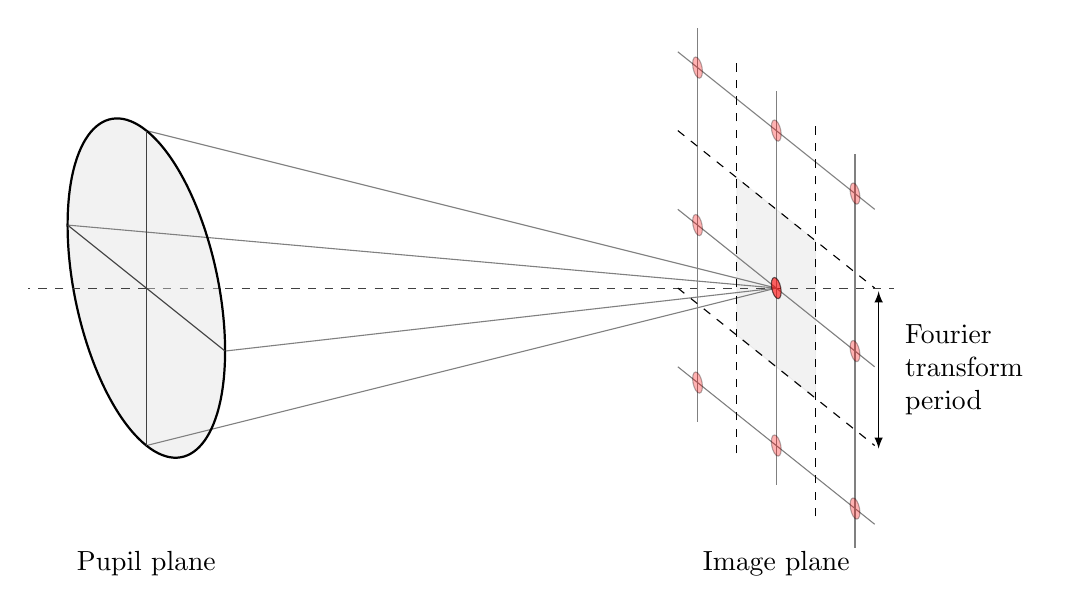
\begin{tikzpicture}[z={(1cm,0cm)},x={(0.5cm,-0.4cm)}, y={(0cm,1cm)}, scale=1]

    % constants
    \def\zimg{8}
    
    % coordinate system 
    \coordinate (0) at (0,0,0);
    \coordinate (2) at (0,0,\zimg);
   
    % optical axis
    \draw[dashed, color=gray] (0) -- +(0,0,1);
    \draw[dashed, color=darkgray] (0,0,1) -- (0,0,9.5);
    

    % Aperture plane
    \draw[color=gray] (-2,0,0) -- (0,0,\zimg);
    \draw[color=gray] (2,0,0) -- (0,0,\zimg);
    \draw[color=gray] (0,-2,0) -- (0,0,\zimg);
    \draw[color=gray] (0,2,0) -- (0,0,\zimg);
    
    \draw[thick, fill=gray, fill opacity=0.1] (0,0) circle [radius=2];
    \draw[color=darkgray] (-2,0,0) -- (2,0,0);
    \draw[color=darkgray] (0,-2,0) -- (0,2,0);
    
    \draw[dashed, color=darkgray] (0) -- +(0,0,-1.5);  % left side of optical axis

    \node [align=left] at (0,-3.5,0) {Pupil plane};

    % Observation plane 
    \draw [fill=gray, fill opacity=0.1, draw=gray, draw opacity=0.1] (-1,-1,\zimg) -- (1,-1,\zimg) -- (1,1,\zimg) -- (-1,1,\zimg) -- cycle;
    %\draw [fill=gray,fill opacity=0.1, draw=gray, draw opacity=0.1] (-2.5,-2.5,\zimg) -- (2.5,-2.5,\zimg) -- (2.5,2.5,\zimg) -- (-2.5,2.5,\zimg) -- cycle; 
    \draw[color=gray] (-2.5,0,\zimg) -- (2.5,0,\zimg);
    \draw[color=gray] (0,-2.5,\zimg) -- (0,2.5,\zimg);
    \draw[color=gray] (-2.5,2,\zimg) -- (2.5,2,\zimg);
    \draw[color=gray] (-2,-2.5,\zimg) -- (-2,2.5,\zimg);
    \draw[color=gray] (-2.5,-2,\zimg) -- (2.5,-2,\zimg);
    \draw[color=gray] (2,-2.5,\zimg) -- (2,2.5,\zimg);
    
    \draw[dashed] (-2.5,-1,\zimg) -- (2.5,-1,\zimg);
    \draw[dashed] (-2.5,1,\zimg) -- (2.5,1,\zimg);
    \draw[dashed] (-1,-2.5,\zimg) -- (-1,2.5,\zimg);
    \draw[dashed] (1,-2.5,\zimg) -- (1,2.5,\zimg);

    % Fourier transform period

    \draw[latex-latex] (2.6,-1,\zimg) -- (2.6,1,\zimg);

    \node [align=center, right] at (2.6,0,\zimg) {\begin{tabular}{l} Fourier\\ transform \\period \end{tabular}};

    \node [align=center] at (0,-3.5,\zimg) {Image plane};
    
    % psf location
    \draw[fill=red, opacity=0.6] (0,0,\zimg) circle [radius=0.125];
    \draw[fill=red, opacity=0.3] (2,2,\zimg) circle [radius=0.125];
    \draw[fill=red, opacity=0.3] (-2,2,\zimg) circle [radius=0.125];
    \draw[fill=red, opacity=0.3] (-2,-2,\zimg) circle [radius=0.125];
    \draw[fill=red, opacity=0.3] (2,-2,\zimg) circle [radius=0.125];
    \draw[fill=red, opacity=0.3] (0,2,\zimg) circle [radius=0.125];
    \draw[fill=red, opacity=0.3] (0,-2,\zimg) circle [radius=0.125];
    \draw[fill=red, opacity=0.3] (2,0,\zimg) circle [radius=0.125];
    \draw[fill=red, opacity=0.3] (-2,0,\zimg) circle [radius=0.125];
    
\end{tikzpicture}

\end{document}
